\chapter{Združené rozdelenie pravdepodobnosti}\label{sec:joint_dist}

V predchádzajúcich kapitolách sme sa zaoberali modelovaním rozdelenia pravdepodobnosti jednej náhodnej premennej, či už jednotlivo alebo v závislosti od ďalších premenných, ktoré už nemusia byť náhodné (regresia a klasifikácia). V praxi sú však prípady, kedy potrebujeme popísať vzájomné správanie niekoľkých náhodných premenných. Na to slúži tzv. \textit{združené rozdelenie pravdepodobnosti}.

Ak premenné modelujeme ako komponenty náhodného vektora $\vec{X} = (X_1, X_2)$, potom znalosť ich združeného rozdelenia nám umožňuje odvodiť ďalšie dôležité vlastnosti systému – napríklad ako vyzerajú podmienené alebo marginálne rozdelenia, prípadne  asymetrie a chvostové závislosti v systéme.

Presné vyjadrenie alebo odhad združeného rozdelenia je však zložitý, čo je podnecované vyšším počtom premenných. S rastúcim rozmerom vektora náhodných premenných rastie aj počet parametrov a miera závislosti, ktorú je potrebné zohľadniť. Preto sa častokrát používajú zjednodušujúce predpoklady, napríklad o nezávislosti alebo naopak špecifickej štruktúre závislosti medzi premennými. My sa budeme zaoberať modelovaním združeného rozdelenia dvoch náhodných premenných.

V tejto kapitole sa zameriame na:
\begin{itemize}
  \item základy modelovania združeného rozdelenia, vrátane podmienených a marginálnych funkcií,
  \item rozklad združeného rozdelenia na marginálne rozdelenia a kopulovú funkciu,
  \item praktické aspekty odhadu združeného rozdelenia na základe dostupných údajov.
\end{itemize}

Konkrétne budeme v tejto kapitole pracovať so združenými rozdeleniami náhodných premenných rovnakého typu – teda buď čisto spojitými, alebo čisto diskrétnymi. Budeme rozoberať všeobecné princípy modelovania, analýzy a odhady takýchto rozdelení. Praktické príklady budú vychádzať z regresných a klasifikačných kontextov, kde sa využívajú znalosti o marginálnych a podmienených rozdeleniach. Pre ilustráciu štruktúry dát a závislostí medzi premennými využijeme nástroje popisnej štatistiky a vizualizačné techniky, ktoré sú súčasťou výstupov mnou implementovanej interaktívnej aplikácie. Táto aplikácia predstavuje aplikačnú časť tejto bakalárskej práce a poskytuje praktické vizualizačné a analytické nástroje na skúmanie združených rozdelení pravdepodobnosti, ktoré sú využité aj pri prezentácii výsledkov v tejto kapitole. Ako ilustračný príklad využívame dataset \textit{Palmer Penguins}~\parencite{horst2020palmerpenguins}, ktorý obsahuje morfologické údaje o troch druhoch tučniakov (Adélie, Chinstrap a Gentoo) žijúcich na ostrovoch Antarktídy. Dataset zahŕňa nasledujúce premenné:

\begin{itemize}
  \item \textit{species} – \textit{Druh}: \texttt{Adelie}, \texttt{Chinstrap}, \texttt{Gentoo}.
  \item \textit{island} – \textit{Ostrov ako miesto výskytu}: \texttt{Biscoe}, \texttt{Dream}, \texttt{Torgersen}.
  \item \textit{culmen\_length\_mm} – \textit{Dĺžka zobáka v milimetroch} (mm): spojitá premenná, v rozsahu približne 32 až 60 mm.
  \item \textit{culmen\_depth\_mm} – \textit{Hĺbka zobáka v milimetroch} (mm): spojitá premenná, približne v rozsahu 13 až 21 mm.
  \item \textit{flipper\_length\_mm} – \textit{Dĺžka plutvy v milimetroch} (mm): spojitá premenná, približne od 170 do 230 mm.
  \item \textit{body\_mass\_g} – \textit{Hmotnosť v gramoch} (g): spojitá premenná, pohybuje sa v rozmedzí 2700 až 6300 g.
  \item \textit{sex} – \textit{Pohlavie}: \texttt{male}, \texttt{female}.
\end{itemize}

Modelovanie zmesi spojitých a diskrétnych náhodných premenných, ako špecifický prípad heterogénnych štruktúr, bude predmetom samostatnej podkapitoly, keďže ide o hlavnú problematiku, na ktorú sa v tejto práci chceme zamerať. Avšak bez ohľadu na typ premenných platí, že združené rozdelenie poskytuje kompletný popis ich spoločného správania a tvorí základ pre odvodenie marginálnych a podmienených rozdelení, ako aj závislostí medzi premennými.


\section{Základy modelovania}\label{sec:joint_zaklady_modelovania}

\subsection{Funkčná reprezentácia}\label{subsec:joint_representation}

Podobne ako to bolo v jednorozmernom prípade, aj viacrozmerné združené rozdelenie možno reprezentovať rôznymi funkciami. My sa v tejto práci budeme zaoberať iba dvojrozmerným prípadom. Dve náhodné premenné $X_1$ a $X_2$ sú najčastejšie charakterizované združenou pravdepodobnostnou funkciou, hustotou alebo distribučnou funkciou, a to v závislosti od typu premenných a existencie uzavretej podoby funkčného vzťahu.

\subsubsection{Hustota pravdepodobnosti}\label{subsec:joint_pdf}

V prípade diskrétnych premenných sa namiesto hustoty používa \textit{združená pravdepodobnostná funkcia} (angl. joint probability mass function), ktorá každému páru hodnôt $(x_1, x_2)$ priraďuje konkrétnu pravdepodobnosť výskytu: 

\begin{equation}
p(x_1, x_2) = \mathrm{Pr}(X_1 = x_1,\, X_2 = x_2)
\end{equation}

Táto pravdepodobnosť je daná explicitne pre jednotlivé kombinácie hodnôt, pričom platí:

\begin{equation}
\sum_{x_1} \sum_{x_2} p(x_1, x_2) = 1
\end{equation}

\begin{figure}[H]
    \centering
    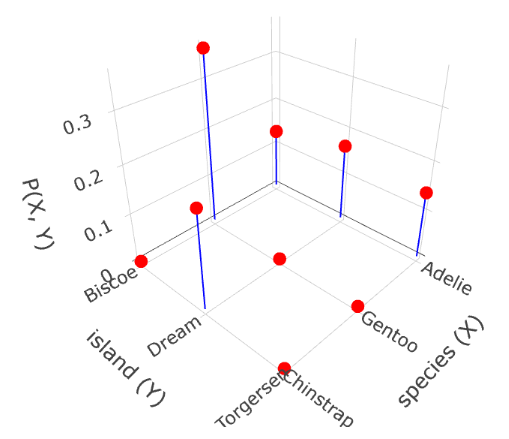
\includegraphics[width=0.7\linewidth]{SK_verzia_praca/figures/pravdeb_funk_ostrov_druhy_3D.png}
    \caption{Pravdepodobnosti premenných \textit{Ostrov ako miesto výskytu} a \textit{Druh} tučniakov.}
    \label{fig:miesto_druh_joint_density}
\end{figure}

Ak sú premenné spojité, spoločné rozdelenie opisujeme prostredníctvom \textit{združenej hustoty pravdepodobnosti} $f$ (angl. joint probability density function – PDF), ktorá udáva pravdepodobnostnú hustotu výskytu dvojice hodnôt v danej oblasti roviny $\mathbb{R}^2$.
Zatiaľ čo v jednorozmernom spojitom prípade nás zaujímala pravdepodobnosť výskytu náhodnej premennej v určitej oblasti na reálnej osi, v prípade dvoch spojitých premenných nás už zaujíma pravdepodobnosť, že obe premenné sa súčasne zrealizujú do danej oblasti v rovine $\mathbb{R}^2$.

Ak $R_1 = [x_1, x_1 + dx_1]$ a $R_2 = [x_2, x_2 + dx_2]$ sú malé intervaly okolo bodu $(x_1, x_2)$, potom pravdepodobnosť, že náhodný vektor $(X_1, X_2)$ spadne do oblasti $R_1 \times R_2$, je približne:

\begin{equation}
\mathrm{Pr}(x_1 \leq X_1 \leq x_1 + dx_1,\ x_2 \leq X_2 \leq x_2 + dx_2) \approx f(x_1, x_2) \, dx_1 \, dx_2
\end{equation}

kde $f(x_1, x_2)$ je hodnota združenej hustoty pravdepodobnosti v bode $(x_1, x_2)$.

Presnejšie, pravdepodobnosť, že sa realizácie oboch premenných nachádzajú v oblasti $[a_1, b_1] \times [a_2, b_2] \in R^2$, vypočítame pomocou dvojnásobného integrálu:

\begin{equation}
\mathrm{Pr}(a_1 \leq X_1 \leq b_1,\ a_2 \leq X_2 \leq b_2) = \int_{a_2}^{b_2} \int_{a_1}^{b_1} f(x_1, x_2) \, dx_1 \, dx_2
\end{equation}

Aby funkcia $f(x_1, x_2)$ bola platnou hustotou pravdepodobnosti, musí platiť:

\begin{equation}
\iint_{\mathbb{R}^2} f(x_1, x_2) \, dx_1 \, dx_2 = 1
\end{equation}

Združené rozdelenie popisuje spoločné správanie dvoch spojitých náhodných premenných a tvorí základ pre ďalšie koncepty ako sú marginálne a podmienené rozdelenia.

Na nasledujúcom obrázku môžeme vidieť príklad vizualizácie združenej hustoty pravdepodobnosti dvoch premenných, pričom ako model výpočtu tu používame jadrové vyhladzovanie (kap.~\ref{textbf:kernel_smoothing}).

\begin{figure}[htpb]
    \centering
    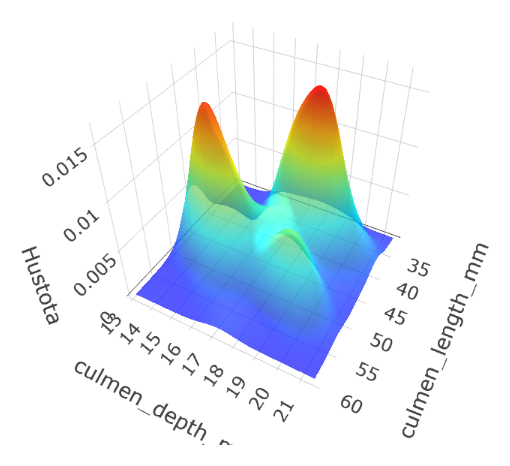
\includegraphics[width=0.7\linewidth]{hustota_hlbka_dlzka_zobaku_3D}
    \caption{Hustota pravdepodobnosti premenných \textit{Hĺbka zobáku} a \textit{Dĺžka zobáku} tučniakov.}
    \label{fig:zobak_joint_density}
\end{figure}

\subsubsection{Kumulatívna distribučná funkcia (CDF)}\label{subsec:joint_cdf}

Spoločná distribučná funkcia $F(x_1, x_2)$ dvoch náhodných premenných $X_1$ a $X_2$ vyjadruje pravdepodobnosť, že obe premenné nadobudnú súčasne hodnoty najviac $x_1$ a $x_2$:

\begin{equation}
F(x_1, x_2) = \mathrm{Pr}(X_1 \leq x_1,\ X_2 \leq x_2),
\end{equation}

pričom vo vzťahu k združenej hustote dvoch spojitých premenných platia nasledujúce vzťahy:

\begin{equation}
F(x_1, x_2) = \int_{-\infty}^{x_1} \int_{-\infty}^{x_2} f(y_1, y_2) \, dy_1 dy_2
\end{equation}

\subsection{Momentové charakteristiky}\label{joint_moments}

Rovnako ako v jednorozmernom prípade, aj v prípade viacrozmerných náhodných veličín (náhodného vektora) sú základnými charakteristikami rozdelenia \textit{stredná hodnota} a \textit{rozptyl}, pričom tentokrát si zavedieme aj pojmy \textit{kovariancie} a \textit{korelačného koeficientu}.

\subsubsection{Stredná hodnota}\label{subsubsec:joint_mean}

Pre náš dvojrozmerný náhodný vektor \(\vec{X} = (X_1, X_2)\) definujeme vektor stredných hodnôt ako:

\begin{equation}
\mathbb{E}[\vec{X}] = \left( \mathbb{E}[X_1], \mathbb{E}[X_2] \right)
\end{equation}

Pre obidva komponenty ho môžeme vyjadriť pomocou marginálnej hustoty (kap.~\ref{subsec:marginal_dist}). Napríklad pre \(X_1\) a marginálnu hustotu \(f_1(x_1)\) platí:

\begin{equation}
\mathbb{E}[X_1] = \int_{\mathbb{R}} x_1 \, f_1(x_1) \, dx_1
\end{equation}

alebo pomocou združenej hustoty:

\begin{equation}
\mathbb{E}[X_1] = \iint_{\mathbb{R}^2} x_1 \, f(x_1, x_2) \, dx_1 \, dx_2
\end{equation}

V prípade, že \(X_1\) je diskrétna náhodná premenná nad množinou hodnôt \(\{x_1^{(i)}\}_{i=1}^{n}\), definujeme jej strednú hodnotu ako:

\begin{equation}
\mathbb{E}[X_1] = \sum_{i=1}^{n} x_1^{(i)} \cdot \Pr(X_1 = x_1^{(i)}),
\end{equation}

kde \(\Pr(X_1 = x_1^{(i)})\) je pravdepodobnostná funkcia diskrétnej premennej \(X_1\).

\subsubsection{Rozptyl}\label{subsubsec:joint_variance}

Rozptyl (disperzia) je definovaný ako očakávaná kvadratická odchýlka od strednej hodnoty:

\begin{equation}
\mathrm{Var}[X_1] = \mathbb{E}[(X_1 - \mathbb{E}[X_1])^2]
\end{equation}

Alternatívne možno rozptyl zapísať aj ako rozdiel momentov:

\begin{equation}
\mathrm{Var}[X_1] = \mathbb{E}[X_1^2] - (\mathbb{E}[X_1])^2
\end{equation}

\subsubsection{Kovariancia}\label{subsubsec:joint_covariance}

Kovariancia vyjadruje mieru lineárnej závislosti medzi dvoma náhodnými premennými \(X_1\) a \(X_2\). Definujeme ju ako:

\begin{equation}
\mathrm{Cov}[X_1, X_2] = \mathbb{E}[(X_1 - \mathbb{E}[X_1])(X_2 - \mathbb{E}[X_2])]
\end{equation}

Kovariancia sa dá alternatívne vyjadriť aj pomocou spoločného momentu:

\begin{equation}
\mathrm{Cov}[X_1, X_2] = \mathbb{E}[X_1 X_2] - \mathbb{E}[X_1] \cdot \mathbb{E}[X_2]
\end{equation}

Tieto hodnoty sa sumarizujú do dvojdimenzionálnej \textit{kovariančnej matice} \(\Sigma\), ktorá je symetrická a pozitívne semidefinitná:

\begin{equation}
\Sigma = 
\begin{bmatrix}
\mathrm{Var}[X_1] & \mathrm{Cov}[X_1, X_2] \\
\mathrm{Cov}[X_2, X_1] & \mathrm{Var}[X_2] \\
\end{bmatrix}
\end{equation}

Kovariančná matica je nevyhnutným nástrojom pre analýzu rozptylu a závislostí medzi komponentami náhodného vektora. Využíva sa napríklad pri odhade parametrov v lineárnej regresii alebo v diskriminačnej analýze.

\subsubsection{Korelačný koeficient}\label{subsubsec:correlation}

Aj keď kovariancia $\mathrm{Cov}[X_1, X_2]$ vyjadruje spoločnú variabilitu dvoch náhodných premenných $X_1$ a $X_2$, jej interpretácia môže byť problematická, pretože jej hodnota závisí od mierky jednotlivých premenných. Teda rovnaká úroveň závislosti medzi premennými môže viesť k rôznym hodnotám kovariancie, ak sú tieto premenné škálované rozdielne.

Túto nevýhodu rieši tzv. \textit{Pearsonov korelačný koeficient}, ktorý je definovaný ako normalizovaná kovariancia:

\begin{equation}
\rho(X_1, X_2) = \frac{\mathrm{Cov}[X_1, X_2]}{\sqrt{\mathrm{Var}[X_1] \cdot \mathrm{Var}[X_2]}}
\end{equation}

Hodnota $\rho(X_1, X_2)$ leží vždy v intervale $[-1, 1]$, pričom:

\begin{itemize}
  \item $\rho = 1$ znamená úplnú pozitívnu lineárnu závislosť,
  \item $\rho = -1$ znamená úplnú negatívnu lineárnu závislosť,
  \item $\rho = 0$ znamená žiadnu lineárnu závislosť (lineárna nezávislosť).
\end{itemize}

Dôležité je, že korelačný koeficient (rovnako ako kovariancia) meria iba \textit{lineárnu} závislosť medzi premennými. Nulová korelácia teda neznamená, že premenné sú nezávislé, ale len to, že medzi nimi nie je lineárny vzťah. Naopak, ak sú dve premenné nezávislé, ich kovariancia aj korelácia sú vždy nulové.

\subsection{Marginálne rozdelenie}\label{subsec:marginal_dist}

Ak nás nezaujíma spoločné správanie všetkých náhodných premenných vektorovej premennej $\vec{X} = (X_1, X_2)$, ale iba jedného jej komponentu, môžeme skúmať jej vlastné pravdepodobnostné rozdelenie. Takéto rozdelenie nazývame \textit{marginálne rozdelenie} (angl. marginal distribution).

Na vizualizáciu marginálneho rozdelenia danej premennej, napríklad $X_2$, môžeme premietnuť každý bod z roviny $(x_1, x_2)$ na os $x_2$ a zostrojiť tak histogram týchto projekcií. Výsledný histogram, po normalizácii tak, aby plocha všetkých stĺpcov bola rovná 1, poskytuje empirický odhad marginálneho rozdelenia $X_2$.

\begin{figure}[H] 
    \centering 
    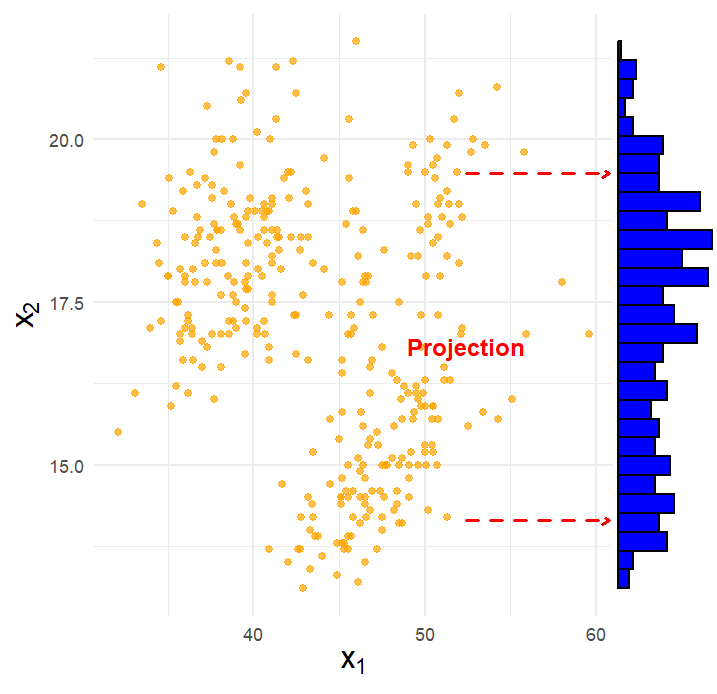
\includegraphics[width=0.7\linewidth]{marg_proj_hist.png} 
    \caption{Empirický odhad marginálneho rozdelenia premennej $X_2$} 
    \label{fig:margin_proj} 
\end{figure}

Z iného pohľadu, marginálne rozdelenie premennej $X_2$ vyjadruje pravdepodobnosť, že hodnota $X_2$ spadne do veľmi úzkeho intervalu $[x_2, x_2 + dx_2]$. V kontexte dvojrozmerného bodového grafu to zodpovedá pravdepodobnosti, že sa bod $(x_1, x_2)$ nachádza v horizontálnom páse výšky $dx_2$.

\begin{figure}[H]
    \centering
    \begin{subfigure}[b]{0.48\linewidth}
        \centering
        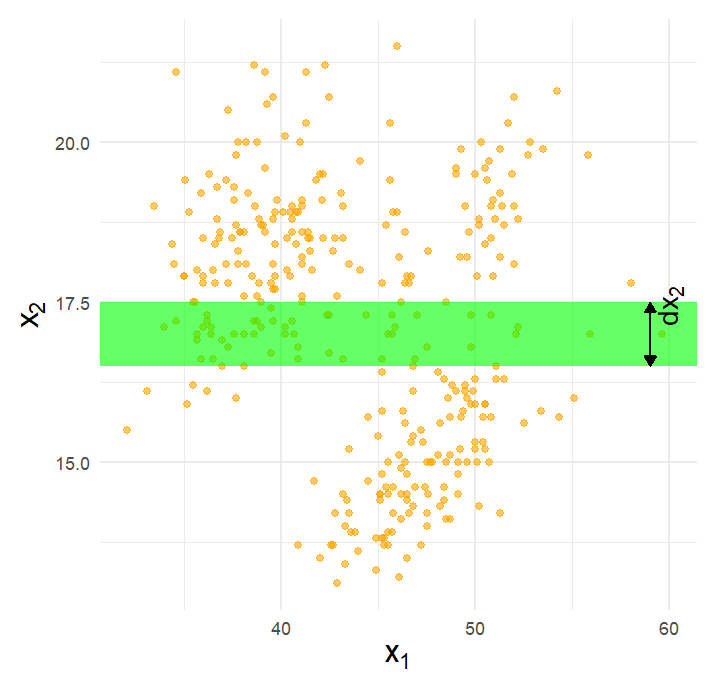
\includegraphics[width=\linewidth]{marg_strip_sum1.png}
        \caption{Horizontálny pás šírky $dx_2$ reprezentujúci interval pre $X_2$.}
        \label{fig:marg_strip_a}
    \end{subfigure}
    \hfill
    \begin{subfigure}[b]{0.48\linewidth}
        \centering
        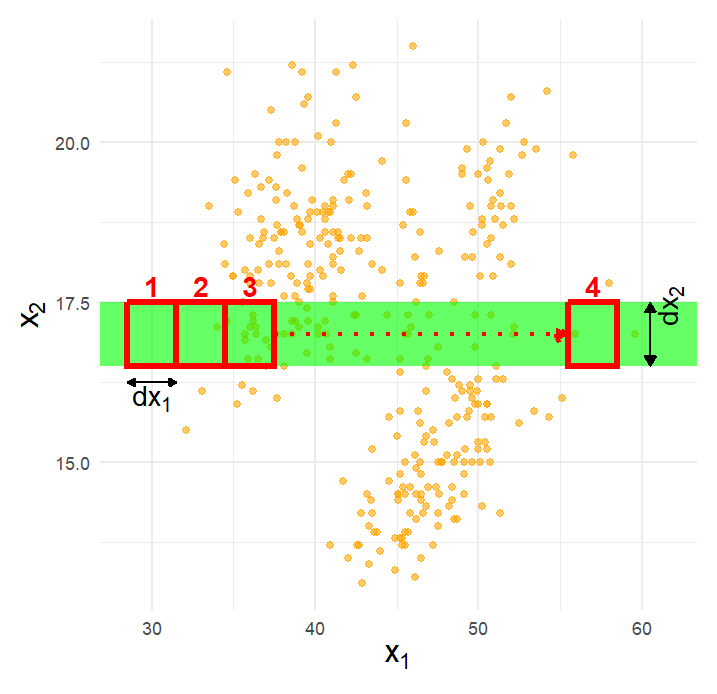
\includegraphics[width=\linewidth]{marg_strip_sum2.png}
        \caption{Pás rozdelený na plôšky $dx_1 \cdot dx_2$, z ktorých sa skladá marginálne rozdelenie $X_2$.}
        \label{fig:marg_strip_b}
    \end{subfigure}
    \caption{Vizuálna interpretácia marginálneho rozdelenia premennej $X_2$}
    \label{fig:marg_strip}
\end{figure}

Ak si pás rozdelíme na plôšky $dx_1 \cdot dx_2$  (Obr.~\ref{fig:marg_strip_b}), potom z nich váženým súčtom dostaneme:

\begin{equation}
\mathrm{Pr}(x_2 \leq X_2 \leq x_2 + dx_2) \approx \sum_i f(x_1^{(i)}, x_2) \, dx_1 \, dx_2
\end{equation}

Porovnaním so vzťahom pre jednorozmernú hustotu pre spojité premenné nám vychádza vzťah, ktorý hovorí o tom, že marginálne rozdelenie $X_2$ možno získať z hustoty združeného rozdelenia $f(x_1, x_2)$ integráciou cez všetky hodnoty $x_1$:

\begin{equation} f_2(x_2) = \int_{-\infty}^{\infty} f(x_1, x_2) dx_1 \end{equation}

Podobne marginálne rozdelenie premennej $X_1$ získame ako:

\begin{equation} f_1(x_1) = \int_{-\infty}^{\infty} f(x_1, x_2)  dx_2 \end{equation}

Tieto marginálne rozdelenia slúžia ako základ pre rozklad združeného rozdelenia (ale aj pre podmieňovanie pravdepodobnosti) pomocou kopúl, ktorému sa budeme venovať v samostatnej podkapitole.

\begin{figure}[H]
    \centering
    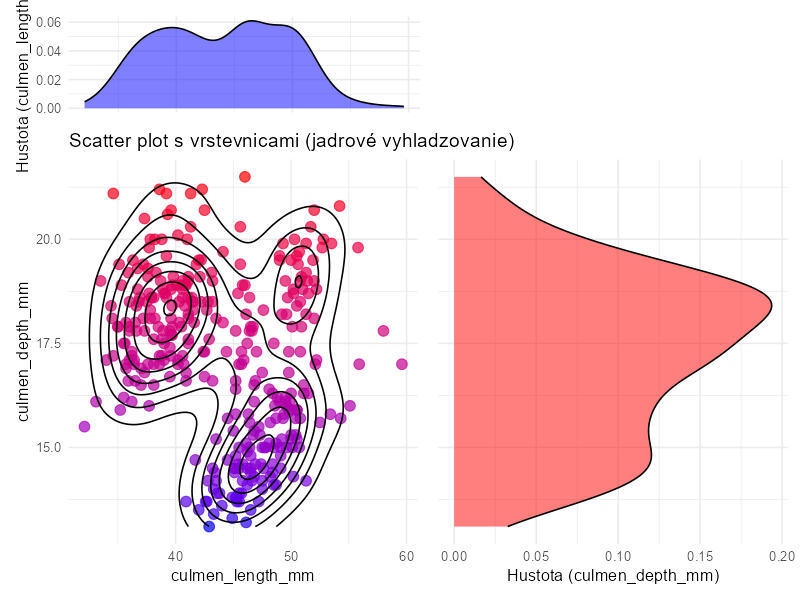
\includegraphics[width=0.8\linewidth]{hustota_hlbka_dlzka_zobaku_2D}
    \caption{Vrstevnice združenej PDF(Obr.~\ref{fig:zobak_joint_density}) + po bokoch marginálne PDF premenných \textit{Hĺbka zobáku} a \textit{Dĺžka zobáku} tučniakov (metóda: jadrové vyhladzovanie ~\ref{textbf:kernel_smoothing})}
    \label{fig:zobak_marg_density}
\end{figure}

\subsection{Podmienené rozdelenie}\label{subsec:conditional_distribution}

Kým marginálne rozdelenie opisuje správanie jednej premennej bez toho aby sa bral do úvahy vplyv ostatných premenných na túto premennú, v mnohých praktických situáciách nás zaujíma, ako sa rozdelenie jednej premennej mení v závislosti od známych hodnôt inej premennej. V takýchto prípadoch hovoríme o \textit{podmienenom rozdelení}.

\subsubsection{Hustota}\label{subsubsec:conditional_density}

Formálne, ak máme náhodný vektor $(X_1, X_2)$, potom podmienená hustota premennej $X_2$ vzhľadom na známu hodnotu $X_1 = x_1$ je definovaná ako:

\begin{equation}
f_{2 \mid 1}(x_2 \mid x_1) = \frac{f(x_1, x_2)}{f_1(x_1)},
\end{equation}

kde:
\begin{itemize}
  \item $f(x_1, x_2)$ je združená hustota,
  \item $f_1(x_1) = \int_{-\infty}^{\infty} f(x_1, x_2) \, dx_2$ je marginálna hustota premennej $X_1$.
\end{itemize}

Z definície o podmienenej pravdepodobnosti vyplýva:

\begin{equation}
\mathrm{Pr}(a \leq X_2 \leq b \mid X_1 = x_1) = \int_a^b f_{2 \mid 1}(x_2 \mid x_1) \, dx_2.
\end{equation}

Podmienenú hustotu $f_{2 \mid 1}(x_2 \mid x_1)$ tu taktiež možno intuitívne interpretovať ako hustotu v rámci tenkého vertikálneho pásu, kde náhodná premenná $X_1$ nadobúda hodnoty z intervalu $[x, x + \varepsilon]$ (Obr.~\ref{fig:cond_density_strip}). V tomto pásme vyberieme všetky body, ktoré spadajú do daného intervalu a z nich vytvoríme histogram hodnôt premennej $X_2$, čím získame empirický odhad hustoty $f_{2 \mid 1}(x_2 \mid x \leq X_1 \leq x +\epsilon)$.

Pre lepšiu predstavu je tento postup znázornený na nasledujúcom obrázku:

\begin{figure}[H]
    \centering
    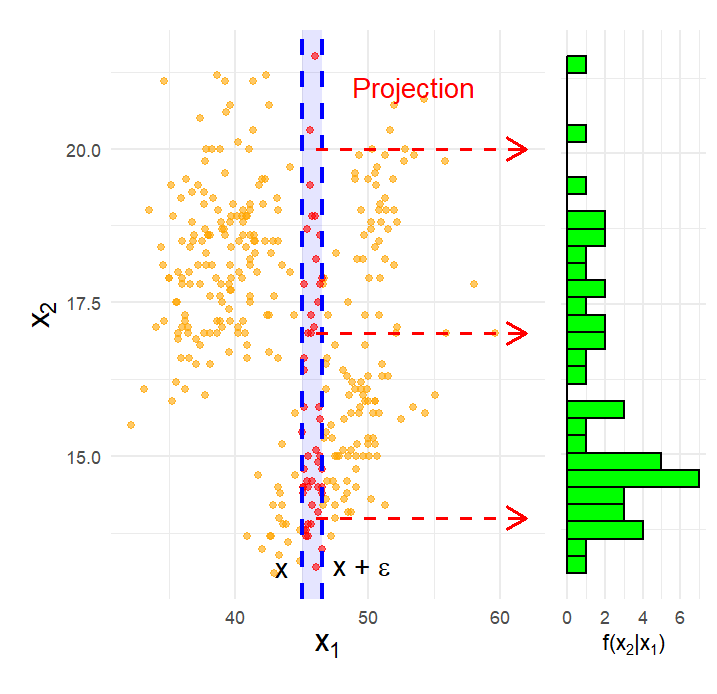
\includegraphics[width=0.7\linewidth]{marg_condition_strip.png}
    \caption{Empirický odhad podmienenej hustoty $f_{2 \mid 1}(x_2 \mid x_1 \in [x, x + \epsilon])$}
    \label{fig:cond_density_strip}
\end{figure}

Týmto sme zaviedli pojem podmienenej hustoty, ktorý bude ďalej kľúčový pri výpočte tzv. \textit{podmienenej strednej hodnoty}. Na ďalšom obrázku môžeme vidieť príklad vizualizácie podmienených hustôt pre spojitú odozvu a prediktor.

\begin{figure}[H]
    \centering
    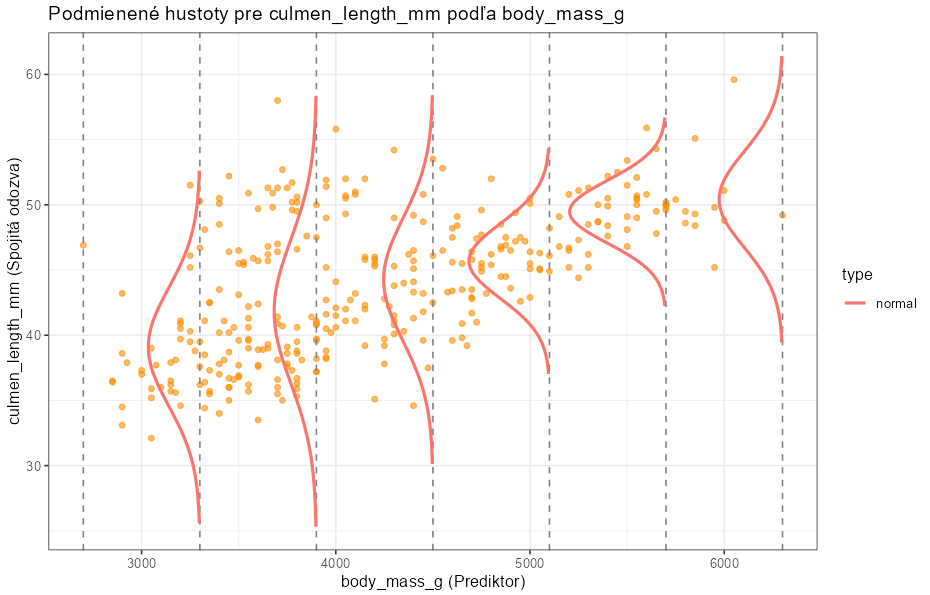
\includegraphics[width=0.8\linewidth]{cond_normal_densities.png}
    \caption{Podmienené hustoty pre premenné (Odozva) $Y=$ \textit{Dĺžka zobáka tučniaka} a (Prediktor) $X=$ \textit{Hmotnosť tučniaka} (parametrický prístup: \textit{normálne rozdelenie}, kap.~\ref{subsubsec:parametric_models})}
    \label{fig:cond_normal_densities}
\end{figure}

\subsubsection{Stredná hodnota}\label{subsubsec:conditional_mean}

Vo všeobecnosti podmienená stredná hodnota vyjadruje očakávanú hodnotu jednej náhodnej premennej vzhľadom na známu hodnotu inej premennej.

Pre diskrétne náhodné premenné $X$ a $Y$ je podmienená stredná hodnota premennej $Y$ vzhľadom na to, že $X = x$, definovaná ako:

\begin{equation}
\mu_{Y|X} = \mathbb{E}[Y|X = x] = \sum_{y} y \cdot \mathrm{Pr}(Y = y \mid X = x)
\end{equation}

Analogicky, ak ide o spojité premenné, tak platí:

\begin{equation}
\mu_{Y|X} = \mathbb{E}[Y|X = x] = \int_{-\infty}^{\infty} y \cdot f_{Y|X}(y \mid x) \, dy
\end{equation}

kde $f_{Y|X}(y \mid x)$, ako už vieme z predošlej podkapitoly, je v tomto prípade podmienená hustota pravdepodobnosti náhodnej premennej $Y$ za predpokladu, že $X = x$.

Podmienená stredná hodnota je teda funkciou známej hodnoty inej premennej a v kontexte regresného modelovania častokrát vystupuje ako regresná funkcia. Napríklad, funkcia $\mu_{Y|X}$ opisuje očakávaný výstup $Y$ vzhľadom na vstup $x$, čo presne zodpovedá určeniu deterministickej zložky regresného modelu.

\subsubsection{Kvantilová funkcia}
\label{subsubsec:conditional_quantile_function}

Pre daný kvantil $q \in (0,1)$ je \textit{podmienená kvantilová funkcia} definovaná ako:
\begin{equation}
Q_{Y \mid X}(q) := \inf \left\{ y \in \mathbb{R} \mid \Pr(Y \leq y \mid X = x) \geq q \right\}
\end{equation}

Táto funkcia vyjadruje, aká hodnota odozvy $Y$ zodpovedá kvantilu $q$ podmieneného rozdelenia vzhľadom na dané hodnoty prediktorov $X = x$. V praxi je túto funkciu potrebné odhadnúť. Existuje viacero prístupov:

\begin{itemize}
  \item odhad cez známe alebo simulované podmienené rozdelenie (napr. zo združeného rozdelenia pomocou marginalizácie),
  \item parametrické modelovanie podmienených kvantilov — napríklad pomocou \textit{kvantilovej regresie}.
\end{itemize}

\medskip
V prípade \textit{lineárnej kvantilovej regresie} sa predpokladá, že kvantilová funkcia má tvar:

\begin{equation}
Q_{Y \mid X}(q) = X^\top \beta_q
\end{equation}

kde $\beta_q$ je vektor parametrov pre daný kvantil $q$. Tento prístup umožňuje skúmať účinok prediktorov nielen na strednú hodnotu, ale aj na ľubovoľný kvantil podmieneného rozdelenia.

Na nasledujúcom obrázku môžeme pozorovať kvantilové funkcie pre vybrané kvantily vo vzťahu k strednej hodnote.

\begin{figure}[H]
    \centering
    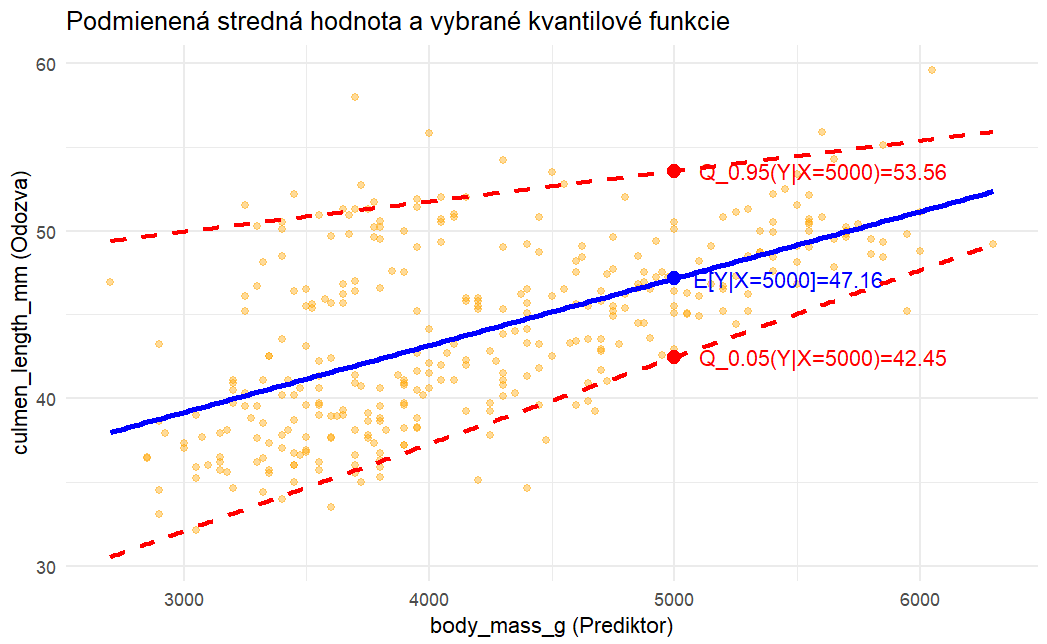
\includegraphics[width=0.8\linewidth]{cond_quant_func.png}
    \caption{Podmienené kvantilové funkcie $Q_{Y \mid X}(0.05)$, $Q_{Y \mid X}(0.95)$ a stredná hodnota $\mathbb{E}[Y \mid X]$ pre premenné $Y=$ \textit{Dĺžka zobáka tučniaka} a $X=$ \textit{Hmotnosť tučniaka} s vypočítanou hodnotou v $X=5000$}
    \label{fig:cond_quant_mean}
\end{figure}

\section{Rozklad rozdelenia spojitých premenných}\label{sec:rozklad_kopule}

Modelovanie spojitého viacrozmerného náhodného vektora nie je vždy efektívne, ak sa snažíme zachytiť spoločné správanie jeho zložiek prostredníctvom jednej parametrickej triedy združeného rozdelenia. Tento prístup totiž neumožňuje samostatne modelovať štruktúru závislosti a vlastností jednotlivých premenných.

Vhodnou alternatívou tu je preto rozklad združeného rozdelenia pravdepodobnosti na dve zložky:
\begin{itemize}
  \item \textit{marginálne rozdelenia} jednotlivých komponentov náhodného vektora,
  \item \textit{kopulu} – funkciu, ktorá tieto marginály spája do jedného celku a zachytáva ich vzájomnú závislosť.
\end{itemize}

Tento prístup formuluje tzv. \textit{Sklarova veta}, ktorá v dvojrozmernom prípade pre každú spojitú distribučnú funkciu $F(x_1, x_2)$ zabezpečuje existenciu unikátnej kopuly $C$, pre ktorú platí:

\begin{equation}\label{eq:copula_dist}
F(x_1, x_2) = C\left(F_1(x_1), F_2(x_2)\right)
\end{equation}

Pre funkciu hustoty dostávame nasledovný rozklad:

\begin{equation}\label{eq:copula_density}
f(x_1, x_2) = c\left(F_1(x_1), F_2(x_2)\right) \cdot f_1(x_1) \cdot f_2(x_2)
\end{equation}

kde $f_1(x_1)$ a $f_2(x_2)$ sú \textit{marginálne hustoty} a $c(u_1, u_2)$ je hustota kopuly.

Tento rozklad nám umožňuje samostatne modelovať:
\begin{itemize}
  \item \textit{tvar individuálnych rozdelení} (napr. normálne, log-normálne, gama, atď.),
  \item \textit{závislosť medzi premennými} prostredníctvom voľby vhodnej kopuly (napr. Gaussova, t-kopula, Claytonova, Gumbelova, atď.).
\end{itemize}

Základom rozkladu podľa \textit{Sklarovej vety} je transformácia pôvodných náhodných premenných $X_i$ pomocou ich marginálnych distribučných funkcií $F_i$, čím sa získa nový vektor $(U_1, U_2)$, kde $U_i = F_i(X_i)$. Výsledné premenné $U_i$ sú potom rovnomerne rozdelené na intervale $[0,1]$, a ich spoločná distribučná funkcia definuje kopulu, ktorá vystihuje štruktúru závislosti nezávisle od tvaru marginálnych rozdelení.

Tento princíp je ilustrovaný na nasledujúcom obrázku:

\begin{figure}[H]
    \centering
    \begin{minipage}{0.45\linewidth}
        \centering
        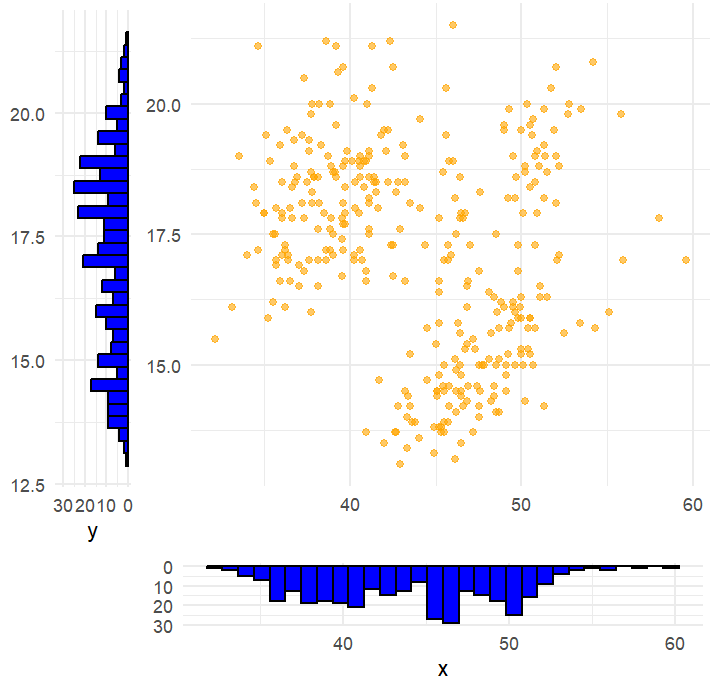
\includegraphics[width=\linewidth]{dist_transform_pred.png}
    \end{minipage}
    \begin{minipage}{0.05\linewidth}
        \centering
        \Huge$\Rightarrow$
    \end{minipage}
    \begin{minipage}{0.45\linewidth}
        \centering
        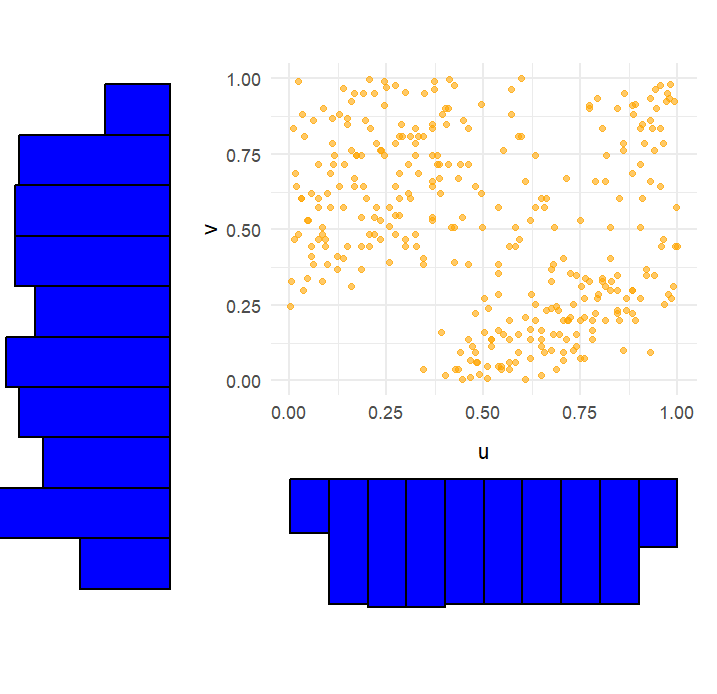
\includegraphics[width=\linewidth]{SK_verzia_praca/figures/dist_transform_po.png}
    \end{minipage}
    \caption{Rozklad združeného rozdelenia: pôvodné hodnoty $(x, y)$ s rôznymi marginálami (vľavo) sú transformované cez $F_1$, $F_2$ na $(u,v)$ (vpravo), ktoré majú rovnomerné rozdelenie na $[0,1]$. Spoločná závislosť sa prenáša do tvaru kopuly.}
    \label{fig:sklar_transform}
\end{figure}

\subsection{Kopula}
\label{subsec:copulas}

Kopula je matematická funkcia, ktorá umožňuje oddeliť modelovanie marginálnych rozdelení od modelovania závislosti medzi náhodnými premennými (pozri~\ref{eq:copula_dist} a ~\ref{eq:copula_density}).

\subsubsection{Vlastnosti}

Každá dvojrozmerná kopula $C: [0,1]^2 \to [0,1]$ musí spĺňať

\begin{itemize}
  \item Hraničné podmienky:
    \begin{align*}
        C(0, u_2) &= 0, \\
        C(u_1, 0) &= 0, \\
        C(1, u_2) &= u_2, \\
        C(u_1, 1) &= u_1.
    \end{align*}
  \item 2-rastúcosť:
  \begin{equation}
    C(v_1, v_2) - C(v_1, u_2) - C(u_1, v_2) + C(u_1, u_2) \geq 0, \quad \text{ak } u_i \leq v_i.
  \end{equation}
\end{itemize}

\subsubsection{Špeciálne prípady}

\begin{itemize}
  \item \textit{Kopula nezávislosti} (produktová):
  \begin{equation}
  \Pi(u_1, u_2) = u_1 u_2.
  \end{equation}
  \item \textit{Kopula úplnej závislosti}:
  \begin{equation}
  M(u_1,u_2) = \min(u_1, u_2).
  \end{equation}
  \item \textit{Kopula úplnej negatívnej závislosti}:
  \begin{equation}
  W(u_1, u_2) = \max(0, u_1 + u_2 - 1).
  \end{equation}
\end{itemize}

Pre dvojrozmerný prípad platí ohraničenie kopuly:
\[
W(u_1, u_2) \leq C(u_1, u_2) \leq M(u_1, u_2).
\]

\subsubsection{Využitie modelu závislosti}

Kopula predstavuje štruktúru závislosti v združenom modeli. Tak ako každá distribučná funkcia, kopula umožňuje napríklad výpočet:

\begin{itemize}
  \item Spoločnej pravdepodobnosti: $\Pr(U_1 \leq u_1,\, U_2 \leq u_2) = C(u_1, u_2)$,
  \item Pravdepodobnosti prekročenia: $\Pr(U_1 > u_1 \vee U_2 > u_2) = 1 - C(u_1, u_2)$,
  \item Podmienených pravdepodobností:
  \[
  \Pr(U_1 \leq u_1 \mid U_2 = u_2) = \frac{\partial C(u_1, u_2)}{\partial u_2}.
  \]
\end{itemize}

\subsubsection{Parametrické triedy}\label{subsubsec:parametric_copula}

\begin{itemize}
  \item \textit{Eliptické kopuly} – napr. Gaussova, t-kopula: modelujú lineárnu závislosť a sú konštruované cez štandardizáciu marginálií eliptických rozdelení:
  
  \begin{equation}
    C_{\Phi}(u_1, u_2) = \Phi\left( \Phi_1^{-1}(u_1), \Phi_2^{-1}(u_2) \right)
  \end{equation}

  \item \textit{Archimedovské kopuly} – napr. Gumbelova, Claytonova, Frankova: jednoduché konštrukcie pomocou generátora $f:[0,1] \to [0,\infty)$:

  \begin{equation}
  C(u_1, u_2) = f^{-1}\left( f(u_1) + f(u_2) \right)
  \end{equation}

  \item \textit{Extreme-value kopuly} – napr. Gumbelova: vhodné pre modelovanie maximálnych javov (napr. povodne). Generované pomocou \textit{dependence function} $\ell : [0, \infty)^2 \rightarrow [0, \infty)$:

  \begin{equation}
  C(u_1, u_2) = \exp\left(-\ell(-\log u_1, -\log u_2)\right)
  \end{equation}
  
\end{itemize}

Pre porovnanie jednotlivých typov kopúl sme si spravili simulácie náhodných výberov, viď obr.~\ref{fig:parametric_copulas}.

\begin{figure}[H]
    \centering
    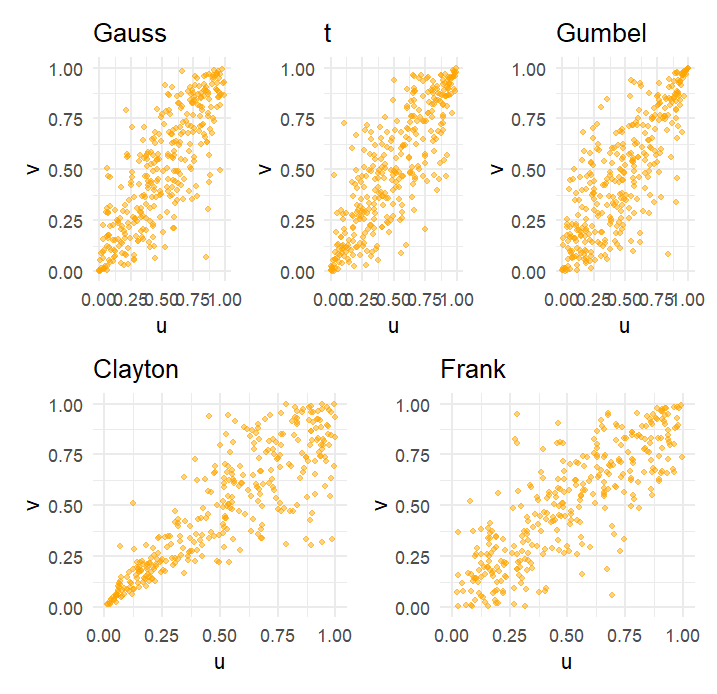
\includegraphics[width=0.95\linewidth]{parametric_copulas.png}
    \caption{Tvar parametrických kopúl pri pevne nastavenej Kendallovej tau $\tau = 0{,}5$.}
    \label{fig:parametric_copulas}
\end{figure}

\subsubsection{Neparametrické triedy}\label{subsubsec:nonparametric_copula}

\textit{Empirická kopula} je neparametrický odhad kopuly vytvorený priamo z dát bez predpokladu konkrétneho tvaru (žiadna Gumbel, Clayton ani t-distribúcia).

Je definovaná ako:

\begin{equation}
C_n(u, v) = \frac{1}{n} \sum_{i=1}^{n} \mathbf{1}\left( \hat{U}^{(i)} \leq u,\ \hat{V}^{(i)} \leq v \right)
\end{equation}

kde $\left(\hat{U}^{(i)}, \hat{V}^{(i)}\right)$ sú \textit{pseudo-pozorovania}, teda dáta transformované pomocou empirických distribučných funkcií (ECDF) na interval $[0,1]$.

\begin{figure}[H]
    \centering
    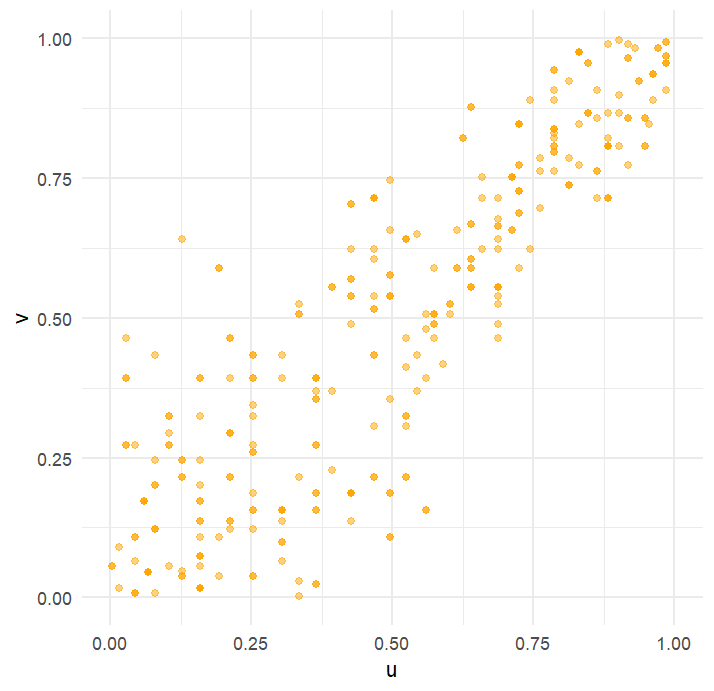
\includegraphics[width=0.6\linewidth]{nonparametric_copula.png}
    \caption{Pseudo-pozorovania premenných \textit{Dĺžka krídiel} a \textit{Hmotnosť} tučniakov}
    \label{fig:nonparametric_copula}
\end{figure}

\section{Modelovanie}\label{sec:modelovanie}

Združené rozdelenie pravdepodobnosti je možné modelovať rôznymi spôsobmi v závislosti od typu údajov, predpokladanej štruktúry a cieľov analýzy. Tak, ako aj v jednorozmernom prípade si tu predstavíme dve hlavné vetvy prístupov: parametrické a neparametrické modely.

\subsection{Parametrické modely}\label{subsec:joint_param_models}

Parametrické modelovanie predpokladá, že združené rozdelenie pravdepodobnosti $\vec{X} = (X_1, X_2)$ patrí do známej triedy rozdelení, určenej vektormi parametrov $\theta \in \Theta$. K takýmto modelom patria:

\begin{itemize}
  \item \textit{Združené normálne rozdelenie} – dvojrozmerné normálne rozdelenie s hustotou
  \begin{equation}
  f_{\mu, \Sigma}(x_1, x_2) = \frac{1}{2\pi |\Sigma|^{1/2}} \exp\left( -\frac{1}{2} (\vec{x} - \vec{\mu})^\top \Sigma^{-1} (\vec{x} - \vec{\mu}) \right),
  \end{equation}
  kde $\vec{\mu} = (\mu_1, \mu_2)^\top$ a $\Sigma$ je symetrická pozitívne definitná kovariančná matica.

   \item \textit{Združené t-rozdelenie} – všeobecnejšie rozdelenie so „zhrubnutými chvostami“ oproti Gaussovskému. Hustota dvojrozmerného t-rozdelenia s $\nu$ stupňami voľnosti je daná:
  \begin{equation}
  f_{\nu, \mu, \Sigma}(x_1, x_2) = \frac{\Gamma\left(\frac{\nu + 2}{2}\right)}{\Gamma\left(\frac{\nu}{2}\right)\nu\pi |\Sigma|^{1/2}} \left[ 1 + \frac{1}{\nu} (\vec{x} - \vec{\mu})^\top \Sigma^{-1} (\vec{x} - \vec{\mu}) \right]^{-\frac{\nu + 2}{2}},
  \end{equation}
  kde $\vec{\mu}$ a $\Sigma$ sú stredná hodnota a kovariančná matica analogicky ako pri normálnom rozdelení, a $\nu > 0$ sú stupne voľnosti.
  
  \item Modely založené na dekompozícii rozdelenia na marginálne rozdelenia $F_1, F_2$ a kopulu $C$, kde sa parametrická forma týka výberu konkrétnej triedy kopuly (napr. Gaussovská, Claytonova, Gumbelova, t-kopula).
\end{itemize}

\subsubsection{Odhad parametrov}\label{subsubsec:param_estimation}

Odhad parametrov $\theta$ pre daný model možno vykonať viacerými spôsobmi, najčastejšie spôsoby sú:

\begin{itemize}
  \item \textit{Metóda momentov} – vychádza z priameho vzťahu medzi teoretickými momentami rozdelenia a jeho parametrami. Tieto momenty sa nahradia empirickými momentami (z výberu) a výsledný súbor rovníc sa vyrieši vzhľadom na neznáme parametre.

  \item \textit{Metóda maximálnej vierohodnosti (Maximum Likelihood)} – tento prístup odhaduje parametre $\theta$ maximalizáciou logaritmickej vierohodnostnej funkcie, ktorá vyjadruje pravdepodobnosť výskytu pozorovanej vzorky vzhľadom na daný model. Formálne:
  \begin{equation}
  \hat{\theta} = \arg\max_{\theta \in \Theta} \frac{1}{n} \sum_{i=1}^{n} \ln f(X_{i1}, X_{i2} \mid \theta)
  \end{equation}
  pričom získané odhady sú konzistentné, efektívne a asymptoticky normálne rozdelené.

  \item \textit{Metóda najmenších štvorcov} – táto metóda vychádza z minimalizácie vzdialenosti medzi teoretickou distribučnou funkciou modelu a jej empirickým odhadom. Napríklad vo forme:
  \begin{equation}
  \hat{\theta} = \arg\min_{\theta \in \Theta} \sum_{i=1}^{n} \left( F(X_{i1}, X_{i2} \mid \theta) - \hat{F}_n(X_{i1}, X_{i2}) \right)^2
  \end{equation}
\end{itemize}

\subsection{Neparametrické modely}\label{subsec:joint_nonparam_models}

Rovnako ako v jednorozmernom prípade, \textit{neparametrické prístupy} nevyžadujú predpoklad o tvare hustoty či distribučnej funkcie, ide o modelovanie založené priamo na dátach. Príklady:

\begin{itemize}
  \item \textit{Empirické združené rozdelenie} – distribučná funkcia $\hat{F}_n(x_1, x_2)$ získaná priamym sčítaním výskytov:
  \begin{equation}
  \hat{F}_n(x_1, x_2) = \frac{1}{n} \sum_{i=1}^{n} \mathbb{I}(X_{i1} \leq x_1, X_{i2} \leq x_2)
  \end{equation}
  \item \textit{Jadrové vyhladzovanie (kernel smoothing)} – pre odhad hustoty $f(x_1, x_2)$:
  \begin{equation}
  \hat{f}_h(x_1, x_2) = \frac{1}{n h_1 h_2} \sum_{i=1}^{n} K\left( \frac{x_1 - X_{i1}}{h_1} \right) K\left( \frac{x_2 - X_{i2}}{h_2} \right)
  \end{equation}
  kde $K$ je vyhladzovacia (jadrová) funkcia (napr. Gaussovská) a $h_j$ sú rozsahy vyhladenia.

  \item \textit{Beta vyhladenie empirickej kopule} (~\ref{subsubsec:nonparametric_copula}) – namiesto ostrého odhadu pomocou indikačnej funkcie sa využíva vyhladzovanie cez beta rozdelenie. Odhad potom vyzerá ako:
  \begin{equation}
    \hat{C}_n^{\beta}(u, v) = \frac{1}{n} \sum_{i=1}^n B(u; r_i, n - r_i + 1) \cdot B(v; s_i, n - s_i + 1)
  \end{equation}
  kde $r_i$ a $s_i$ sú poradia $U_i$ a $V_i$ vo vzorke a $B(\cdot; a,b)$ je kumulatívna distribučná funkcia beta s parametrami a,b.
  
\end{itemize}

\begin{figure}[H]
    \centering
    \begin{minipage}[t]{0.48\linewidth}
        \centering
        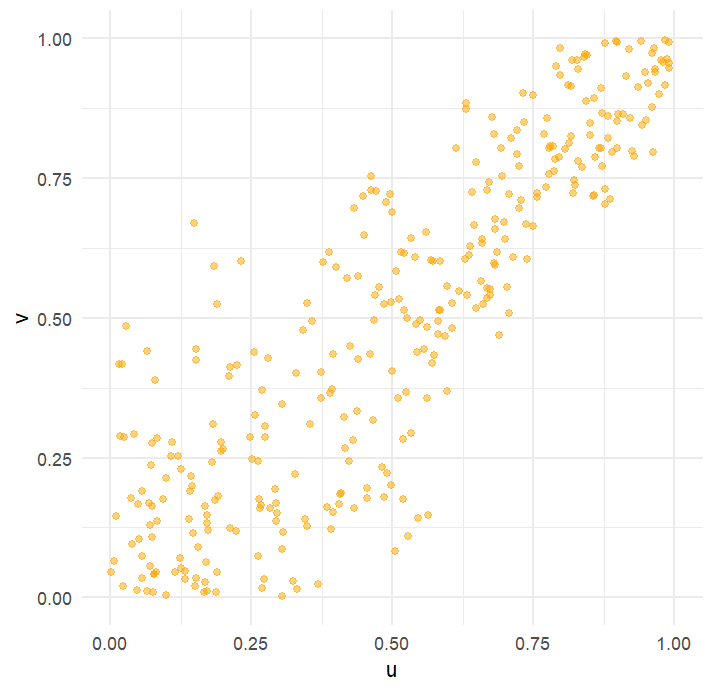
\includegraphics[width=\linewidth]{nonparametric_copula_beta.png}
    \end{minipage}
    \hfill
    \begin{minipage}[t]{0.48\linewidth}
        \centering
        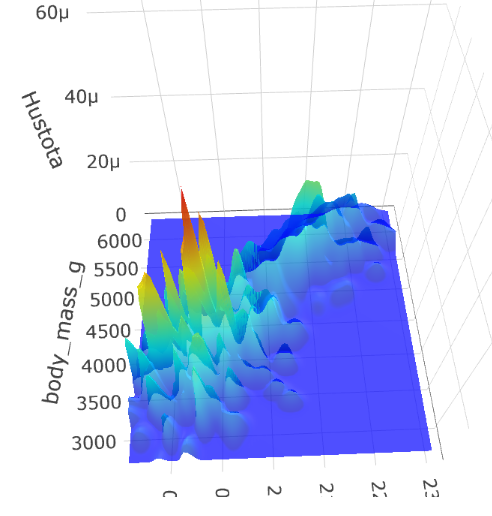
\includegraphics[width=\linewidth]{nonparametric_copula_dens.png}
    \end{minipage}
    \caption{Použitie beta vyhladenej empirickej kopule na modelovanie združeného rozdelenia premenných \textit{Dĺžka krídiel} a \textit{Hmotnosť} tučniakov (vpravo hustota: jadrový odhad marginálií~\ref{eq:kernel_smoothing}, vľavo pseudo-pozorovania)}
    \label{fig:empcopula}
\end{figure}

\section{Modelovanie rozdelenia zmiešaného náhodného vektora}\label{sec:joint_mixture_modeling}

V mnohých praktických aplikáciách sa stretávame so situáciami, kde niektoré komponenty náhodného vektora sú diskrétne, zatiaľ čo iné sú spojité. Takéto náhodné vektory označujeme ako \textit{zmiešané} (angl. \textit{mixed-type random vectors}). Typickým príkladom sú meteorologické, poisťovacie alebo simulačné modely, kde napr. výskyt udalosti je diskrétny, ale jej rozsah je spojitý. 

Modelovanie týchto štruktúr je komplikované najmä preto, že štandardné pravdepodobnostné modely predpokladajú homogénny typ premenných (všetky spojité alebo všetky diskrétne).

\subsection{Prehľad prístupov ku konštrukcii združeného rozdelenia}\label{subsec:overview_joint_mixed}

Podľa práce ~\textcite{pleisMixtureDissertation} môžeme pri tvorbe združeného rozdelenia zmiešaných premenných uvažovať tri základné prístupy:

\subsubsection{Rozklad na podmienené a marginálne rozdelenia}
Ak máme diskrétnu premennú $D$ a spojitú premennú $C$, môžeme využiť základný princíp:

\begin{equation}
f_{D,C}(d, c) = \Pr(D = d) \cdot f_{C \mid D}(c \mid d).
\end{equation}

alebo alternatívne:

\begin{equation}
f_{D,C}(d, c) = f_C(c) \cdot \Pr(D = d \mid C=c).
\end{equation}

Tento prístup možno nazývať ako stratifikované modelovanie, kde každá kategória diskrétnej premennej má svoje vlastné rozdelenie spojitej zložky.


\subsubsection{Modelovanie pomocou kopúl}\label{copula_joint_density}

Jedným z nástrojov, ktoré umožňujú spojiť rozdielne typy premenných v spoločnom modeli, sú \textit{kopule}.

Avšak kopule, ktoré bežne používame (napr. Gaussova alebo t-kopula), sú definované nad spojitými distribučnými funkciami. Pokiaľ aspoň jedna z marginálnych distribúcií nie je spojitá, ako v našom prípade, prestáva platiť jednoznačnosť dekompozície podľa \textit{Sklarovej vety} a výsledná kopula nie je na celom priestore jednoznačne určená.

To vedie k viacerým problémom:
\begin{itemize}
  \item \textit{Problémy na hraniciach} – diskrétne premenné nemajú spojitú distribučnú funkciu, čo vedie k nejednoznačnosti transformácie na jednotkový interval.
  \item \textit{Strata informácie} – binarizácia alebo kódovanie kategoriálnej premennej vedie k strate jemnej štruktúry závislosti.
  \item \textit{Interpretácia} – štruktúra závislosti medzi kategoriálnou a spojitou premennou je pri tomto prístupe ťažko interpretovateľná.
\end{itemize}

Z týchto dôvodov sa v aplikáciách uplatňujú alternatívne stratégie ako napríklad \textit{conditional copula modeling}, kde sa predpokladá, že rozdelenie spojitej premennej $C$ vzhľadom na diskrétnu premennú $D = d$ má vlastnú kopulu, a teda sa modelujú podmienené distribúcie $\mathbb{C}_d$ osobitne pre každú triedu $d$~\parencite{pleisMixtureDissertation}. Tento prístup zároveň umožňuje riešiť problém nejednoznačnosti tým, že sa každá trieda modeluje ako samostatný „blok“ so špecifickou štruktúrou závislosti.

\subsubsection{Latentné premenné}\label{latent_vars}

Latentný prístup modeluje diskrétnu premennú ako \textit{prahovanie (thresholding)} nepozorovanej spojitej veličiny. Tento model je obzvlášť vhodný pre ordinálne premenné, no pre nominálne nemusí byť vždy interpretovateľný alebo vhodný.

Podrobnejšie rozpracovanie týchto techník však presahuje rámec tejto práce a preto sa im ďalej venovať nebudeme.

\subsection{Modelovanie združeného rozdelenia ako kombináciu podmienených hustôt}\label{subsec:glom_joint_mixture}

Pri modelovaní \textit{združeného rozdelenia} zmiešaného náhodného vektora $(D, C)$, kde $D$ je diskrétna (kategoriálna) premenná a $C$ je spojitá, vychádzame z tzv. \textit{general location model} (GLOM), ktorý bol podrobne predstavený v práci ~\textcite{pleisMixtureDissertation} ako vhodný spôsob modelovania zmiešaného vektora pomocou zmesi podmienených Gaussových rozdelení s rovnakým rozptylom. Tento prístup vyjadruje združenú hustotu ako súčin marginálnej pravdepodobnosti diskrétnej premennej a podmienenej hustoty spojitej premennej:

\begin{equation}
f_{D,C}(d, c) = \Pr(D = d) \cdot f_{C \mid D}(c \mid d).
\end{equation}

Z toho následne vyplýva \textit{marginálna hustota spojitej premennej} ako vážený súčet:

\begin{equation}
f_C(c) = \sum_{d=1}^{K} \Pr(D = d) \cdot f_{C \mid D}(c \mid d),
\end{equation}

pričom váhy $\Pr(D = d)$ zodpovedajú výskytom jednotlivých kategórií v dátach a $f_{C \mid D}(c \mid d)$ predstavuje podmienenú hustotu spojitej premennej v rámci danej kategórie.

Analogicky môžeme získať aj \textit{marginálnu pravdepodobnostnú funkciu diskrétnej premennej} $D$ integráciou združenej hustoty nad spojitou premennou $C$:

\begin{equation}
\Pr(D = d) = \pi_d = \int_{\mathbb{R}} f_{D,C}(d, c) \, dc,
\end{equation}

kde $f_{D,C}(d, c)$ je združená hustota zmiešaného náhodného vektora $(D, C)$. Tento vzťah vyjadruje pravdepodobnosť výskytu kategórie $d$ ako celkovú pravdepodobnosť v spojitom priestore $C$ pre dané $D = d$.

V každej diskrétnej triede $D = d$ sa predpokladá vlastné parametrické rozdelenie spojitej zložky $f_{C \mid D=d}(c)$, avšak je možné použiť aj jadrové vyhladzovanie ako neparametrický prístup. Výsledná hustota sa nakoniec zostavuje ako vážená kombinácia podmienených hustôt ktoré môžu byť pre rôzne kategórie odlišné, čím sa prirodzene zohľadňuje ich štrukturálna rozdielnosť.

Tento model možno implementovať nasledovne:
\begin{itemize}
  \item Diskrétna premenná $D$ je kódovaná ako faktor s $K$ kategóriami.
  \item Pre každú kategóriu $d = 1, \dots, K$ sa vypočíta podmienená hustota $f_{C \mid D}(c \mid d)$ – buď neparametricky (jadrovým vyhladzovaním), alebo pomocou parametrov napríklad normálneho alebo Studentovho $t$-rozdelenia.
  \item Každá hustota je následne vážená podľa výskytu kategórie $\pi_d$ v dátach (empirická pravdepodobnosť).
  \item Výsledná hustota $f_C(c)$ je tak zmesou hustôt podmienených výskytom kategórie.
\end{itemize}

Táto stratégia zodpovedá konštrukcii konečnej zmesi:

\begin{equation}
f_C(c) = \sum_{d=1}^{K} \pi_d \cdot f_{C|D=d}(c), \quad \text{kde } \sum_{d=1}^{K} \pi_d = 1.
\end{equation}

Tento prístup má niekoľko výhod oproti metódam, ktoré sa snažia modelovať združené rozdelenie zmiešaných premenných priamo, napríklad pomocou spojitých kopúl alebo binarizáciou kategoriálnej premennej:
\begin{itemize}
  \item Zachováva jemnú štruktúru závislosti medzi $C$ a $D$, bez potreby nepresného binárneho kódovania.
  \item Vyhýba sa problémom pri použití spojitých kopúl na kombináciu diskrétnych a spojitých rozdelení.
  \item Model má prirodzenú generatívnu interpretáciu: najskôr sa podľa pravdepodobnosti $\Pr(D = d)$ vyberie konkrétna hodnota diskrétnej premennej $D$, a následne sa hodnota spojitej premennej $C$ modeluje podmieneným rozdelením $f_{C \mid D}(c \mid d)$. 
\end{itemize}

Na druhej strane, použitie tejto stratégie predpokladá, že pre každú kategóriu $D = d$ je možné spoľahlivo odhadnúť parametre rozdelenia spojitej premennej. V prípade veľmi malých kategórií môže byť však tento odhad nestabilný.

\bigskip

\begin{figure}[H]
    \centering
    \begin{minipage}[t]{0.48\linewidth}
        \centering
        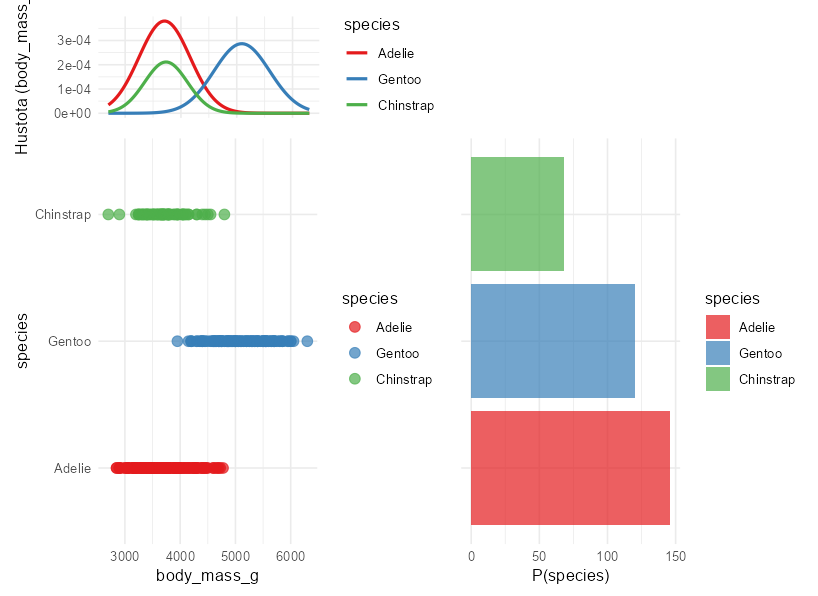
\includegraphics[width=\linewidth]{joint_mixture_density_2D.png}
    \end{minipage}
    \hfill
    \begin{minipage}[t]{0.48\linewidth}
        \centering
        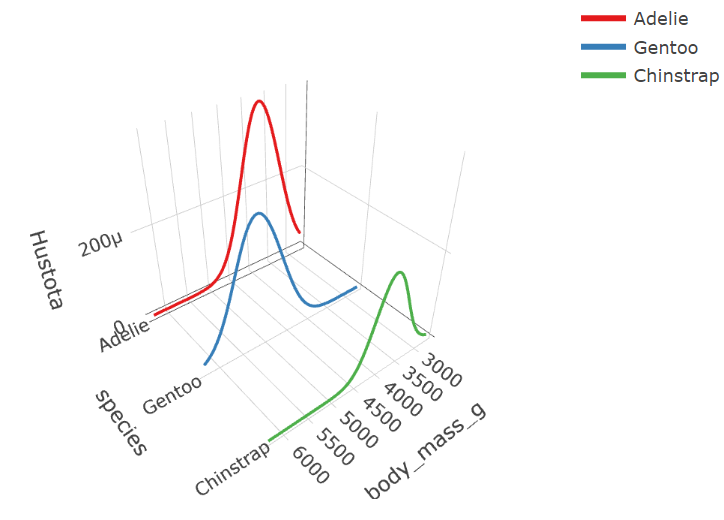
\includegraphics[width=\linewidth]{joint_mixture_density_3D.png}
    \end{minipage}
    \caption{Stratifikované modelovanie združenej hustoty pravdepodobnosti premenných \textit{Druh} a \textit{Hmotnosť} tučniakov (vľavo graf: Pozorovania + Marginálie, vpravo graf: Združená hustota (parametricky: normálne rozdelenie))}
    \label{fig:stratified_modelling_mix_density}
\end{figure}


\subsection{Podmienené rozdelenie}

\subsubsection{Hustota}

Podmienená hustota spojitej premennej $C$ vzhľadom na kategóriu $D=d$ sa vypočíta ako:

\begin{equation}
f_{C \mid D}(c \mid d) = \frac{f_{D,C}(d, c)}{\Pr(D = d)},
\end{equation}

\begin{figure}[H]
    \centering
    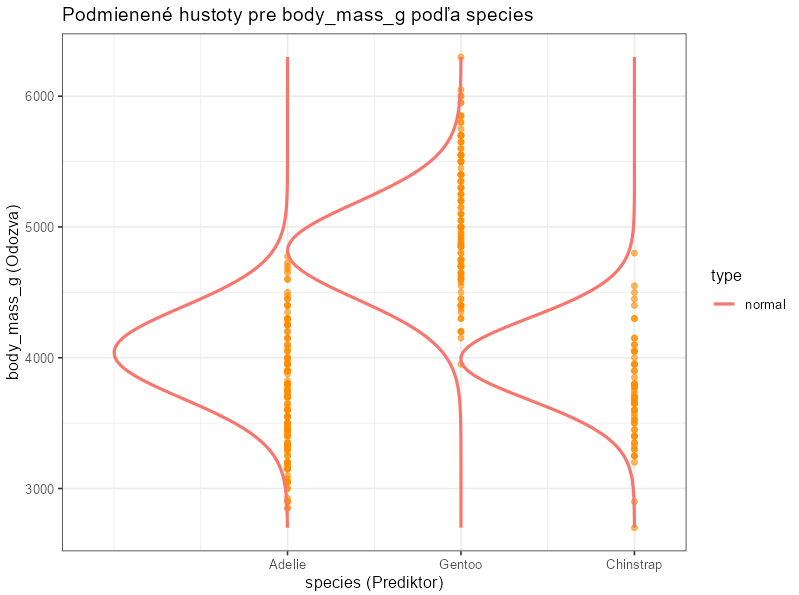
\includegraphics[width=0.8\linewidth]{cond_dens_mix_contresp.png}
    \caption{Podmienená hustota (parametrická: normálne rozdelenie) spojitej premennej \textit{Hmotnosť} vzhľadom na diskrétnu premennú \textit{Druh} tučniakov}
    \label{fig:cond_dens_mix_contresp}
\end{figure}

Podmienenú pravdepodobnostnú funkciu kategórie vzhľadom na spojitú hodnotu počítame nasledovne:

\begin{equation}
\Pr(D = d \mid C = c) = \frac{\Pr(D = d) \cdot f_{C \mid D}(c \mid d)}{f_C(c)}.
\end{equation}

\begin{figure}[H]
    \centering
    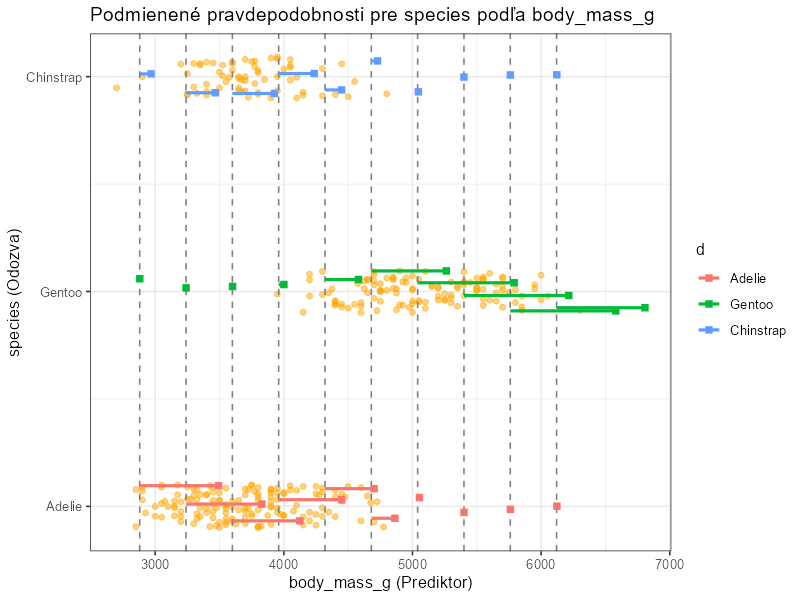
\includegraphics[width=0.8\linewidth]{cond_dens_mix_discresp.png}
    \caption{Podmienená pravdepodobnostná funkcia diskrétnej premennej \textit{Druh} vzhľadom na spojitú premennú \textit{Hmotnosť} tučniakov}
    \label{fig:cond_dens_mix_contresp}
\end{figure}

\subsubsection{Stredná hodnota a kvantilová funkcia}

Podmienená stredná hodnota spojitej premennej vzhľadom na kategóriu $D = d$ je definovaná ako:

\begin{equation}
\mathbb{E}[C \mid D = d] = \int_{\mathbb{R}} c \cdot f_{C \mid D}(c \mid d) \, dc,
\end{equation}

Kvantilová funkcia spojitej premennej $C$ podmienená kategóriou $D = d$:

\begin{equation}
Q_C^{(d)}(q) := \inf \left\{ c \in \mathbb{R} \mid \int_{-\infty}^c f_{C \mid D}(t \mid d) \, dt \geq q \right\}.
\end{equation}

Podmienená stredná hodnota diskrétnej premennej vzhľadom na hodnotu spojitej:

\begin{equation} 
\mathbb{E}[D \mid C = c] = \sum_{k = 1}^{K} d_k \cdot \Pr(D = d_k \mid C = c), \end{equation}

Kvantilová funkcia diskrétnej premennej $D$ vzhľadom na $C = c$:

\begin{equation} 
Q_D^{(c)}(q) := \min \left\{ d_k \in \mathcal{D} \mid \sum_{j=1}^{k} \Pr(D = d_j \mid C = c) \geq q \right\}, 
\end{equation}

kde $\mathcal{D} = \{ d_1, \ldots, d_K \}$ je množina všetkých možných hodnôt diskrétnej premennej $D$.
